%---------------------- Problema 1 ------------------------------
\section*{Problema 1}


La barra de acero ($E = 206$ GPa y $S_y = 300$ MPa) en posici\'on vertical de la Figura ($L = 10$ m) tiene secci\'on transversal variable
\[
A(z) = A_0\, e^{-z/L}, \qquad A_0 = 1600\ \text{mm}^2,
\]
y est\'a sometida a una fuerza axial en su extremo libre ($P = 3$ kN). De acuerdo a la teor\'ia de barras, se pide:

\begin{enumerate}[label=\alph*), itemsep=4pt]
    \item Obtener la expresi\'on anal\'itica de los campos de tensi\'on y desplazamiento axial.
    \item Obtener la soluci\'on por MEF de dichos campos utilizando discretizaciones con 1, 2 y 4 elementos finitos de dos nodos de \'area constante en cada uno de ellos.
    \item Comparar y discutir las soluciones obtenidas en a) y b).
\end{enumerate}

\begin{center}
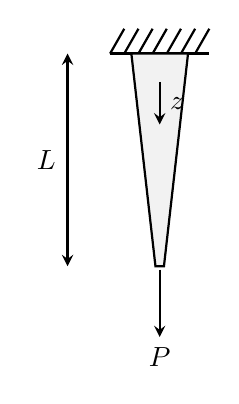
\begin{tikzpicture}[scale=0.9, >=stealth, thick]
    % apoyo empotrado (rayado)
    \draw[thick] (-0.7,3) -- (0.7,3);
    \foreach \x in {-0.7,-0.5,...,0.5}
        \draw (\x,3) -- (\x+0.2,3.35);

    % barra conica (mas ancha arriba, angosta abajo)
    \draw[thick, fill=black!5]
        (-0.4,3) -- (-0.06,0) -- (0.06,0) -- (0.4,3) -- cycle;

    % cota L
    \draw[<->] (-1.3,3) -- (-1.3,0);
    \node at (-1.6,1.5) {$L$};

    % eje z
    \draw[->] (0,2.6) -- (0,2.0);
    \node[right] at (0,2.3) {$z$};

    % carga P
    \draw[->] (0,-0.05) -- (0,-1.0);
    \node[below] at (0,-1.0) {$P$};
\end{tikzpicture}
\end{center}

\vspace{0.7cm}

%---------------------- Desarrollo -------------------------------

\begin{desarrollo}{a) Campos anal\'iticos de tensi\'on y desplazamiento}
    Para poder desarrollar esto lo que tenemos que hacer es un diagrama de la fuerza axial a la que cada parte de la barra se encuentra, para esto hacemos una funcion que la tenga en cuenta. Podemos tener en cuenta la fuerza axial de la barra en cada parte tenemos que saber si consideramos la fuerza peso o no, en caso que no lo contabilicemos se puede expresar asi la fuerza axial
    $$N(z)=3\text{k}N$$
    Con esto podemos calcular el esfuerzo axial
    $$\sigma_z(z)=\dfrac{N(z)}{A(z)}$$
    Una vez teniendo el esfuerzo podemos usar la propiedad constitutiba que relacion el esfuerzo con la deformacion, asumiento esfuerzo uniaxial, no hay efectos de adelgazamiento, tenemos 
    $$\sigma_z=E\varepsilon_z\longrightarrow \varepsilon_z=\dfrac{\sigma_z(z)}{E}=\dfrac{\partial w}{\partial z}$$
    
    $$\sigma_z(z)=\dfrac{3\text{k}N}{A_0e^{-z/L}}\quad \quad \varepsilon_z(z)=\dfrac{3\text{k}N}{EA_0e^{-z/L}}$$ 
    $$\dfrac{\partial w}{\partial z}=\dfrac{3\text{k}N}{EA_0e^{-z/L}}$$ 
    $$\int_{w_i}^{w_f} dw=\int_{\mathcal{B}}\dfrac{3\text{k}N}{EA_0e^{-z/L}}dz$$ 
    $$\delta_z=\dfrac{3000}{206\text{GPa}\cdot1600\text{mm}^2}\int_{\mathcal{B}}e^{z/L}dz$$
    $$\int_{0}^{L} e^{z/L} \, dz = \left[ L e^{z/L} \right]_{0}^{L}$$

$$\left[ L e^{z/L} \right]_{0}^{L} = L e^1 - L e^0 = L(e - 1)$$

$$\delta_z = \frac{3000 \text{N}\cdot 10\text{m}\cdot(e - 1)}{206000\text{MPa} \cdot 1600\text{mm}^2}$$
$$\delta_z \approx 0,1564\text{ mm}$$
\end{desarrollo}
\newpage
\begin{desarrollo}{b) Soluci\'on por MEF}
    \textit{Discretizaci\'on con 1 elemento}\\
    
    Para este caso nosotros tenemos este sistema
 \begin{center}
    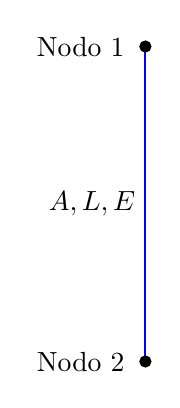
\begin{tikzpicture}
        % Dibujo de la barra
        \draw[thick, blue] (0,0) -- (0,-4)  node[midway, left, black] {$A,L, E$};
        
        % Nodo 1 (Superior)
        \filldraw[black] (0,0) circle (2pt) node[left=4pt] {Nodo 1};
        % Nodo 2 (Inferior)
        \filldraw[black] (0,-4) circle (2pt) node[left=4pt] {Nodo 2};
    \end{tikzpicture}
\end{center}
El cual se puede expresar como un resorte de constante $k=\dfrac{E}{AL}$
queda el balance de cada nodo como
\begin{align*}
    -k(u_2-u_1)&=R_1\\
    -k(u_1-u_2)&=F_1
\end{align*}
En forma matricial se veria asi
$$k\begin{bmatrix}
    1&-1\\
    -1&1
\end{bmatrix}\begin{bmatrix}
    u_1\\
    u_2
\end{bmatrix}=\begin{bmatrix}
    R_1\\
    F_1
\end{bmatrix}$$
Teniendo en cuenta las condiciones iniciales, tenemos que $u_1=0$ y $F_1=3\text{kN}$
Por ende la matriz de rigidez reducida como\\
$$F_1=u_2\cdot k\longrightarrow u_2=\dfrac{F_1}{k}$$
    \\
    \textit{Discretizaci\'on con 2 elementos}
    Para este caso nosotros tenemos este sistema
 \begin{center}
    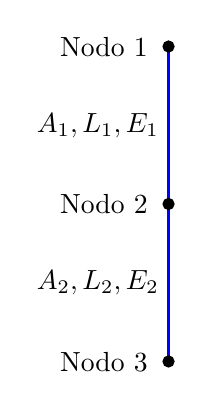
\begin{tikzpicture}
        % Dibujo de la barra
        \draw[thick, blue] (0,0) -- (0,-4);
        \node[left, black] at (0,-1){$A_1,L_1, E_1$};
        \node[left, black] at (0,-3){$A_2,L_2, E_2$};
        % Nodo 1 (Superior)
        \filldraw[black] (0,0) circle (2pt) node[left=4pt] {Nodo 1};
        % Nodo 2 (Inferior)
        \filldraw[black] (0,-2) circle (2pt) node[left=4pt] {Nodo 2};
        \filldraw[black] (0,-4) circle (2pt) node[left=4pt] {Nodo 3};
    \end{tikzpicture}
\end{center}
El cual se puede expresar como un resorte de constante $k=\dfrac{E}{AL}$
queda el balance de cada nodo como
\begin{align*}
    -k_1(u_2-u_1)&=R_1\\
    -k_1(u_1-u_2)-k_2(u_3-u_2)&=0\\
    -k_2(u_2-u_3)&=F_1
\end{align*}
En forma matricial se veria asi
$$\begin{bmatrix}
    k_1&-k_1&0\\
    -k_1&k_1+k_2&-k_2\\
    0&-k_2&k_2
\end{bmatrix}\begin{bmatrix}
    u_1\\
    u_2\\
    u_3
\end{bmatrix}=\begin{bmatrix}
    R_1\\
    0\\
    F_1
\end{bmatrix}$$
Teniendo en cuenta las condiciones iniciales, tenemos que $u_1=0$ y $F_1=3\text{kN}$
Por ende la matriz de rigidez reducida como\\




$$\begin{bmatrix}

k_1+k_2&-k_3\\
-k_3&k_3
\end{bmatrix}\begin{bmatrix}

    u_2\\
    u_3
\end{bmatrix}=\begin{bmatrix}

    0\\
    F_1
\end{bmatrix}$$

    \textit{Discretizaci\'on con 4 elementos}
    Para este caso nosotros tenemos este sistema
 \begin{center}
    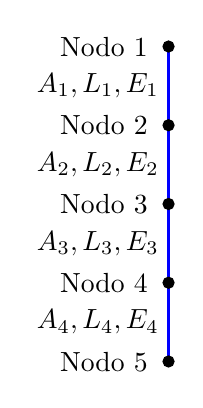
\begin{tikzpicture}
        % Dibujo de la barra
        \draw[thick, blue] (0,0) -- (0,-4);
        \node[left, black] at (0,-0.5){$A_1,L_1, E_1$};
        \node[left, black] at (0,-1.5){$A_2,L_2, E_2$};
        \node[left, black] at (0,-2.5){$A_3,L_3, E_3$};
        \node[left, black] at (0,-3.5){$A_4,L_4, E_4$};
        % Nodo 1 (Superior)
        \filldraw[black] (0,0) circle (2pt) node[left=4pt] {Nodo 1};
        % Nodo 2 (Inferior)
        \filldraw[black] (0,-1) circle (2pt) node[left=4pt] {Nodo 2};
        \filldraw[black] (0,-2) circle (2pt) node[left=4pt] {Nodo 3};
        \filldraw[black] (0,-3) circle (2pt) node[left=4pt] {Nodo 4};
        \filldraw[black] (0,-4) circle (2pt) node[left=4pt] {Nodo 5};
    \end{tikzpicture}
\end{center}
El cual se puede expresar como un resorte de constante $k=\dfrac{E}{AL}$
queda el balance de cada nodo como
\begin{align*}
    -k_1(u_2-u_1)&=R_1\\
    -k_1(u_1-u_2)-k_2(u_3-u_2)&=0\\
    -k_2(u_2-u_3)-k_3(u_4-u_3)&=0\\
    -k_3(u_3-u_4)-k_4(u_5-u_4)&=0\\
    -k_4(u_4-u_5)&=F_1
\end{align*}
En forma matricial se veria asi
$$\begin{bmatrix}
    k_1&-k_1&0&0&0\\
    -k_1&k_1+k_2&-k_2&0&0\\
    0&-k_2&k_2+k_3&-k_3&0\\
    0&0&- k_3&k_3+k_4&-k_4\\
    0&0&0&-k_4&k_4
    
\end{bmatrix}\begin{bmatrix}
    u_1\\
    u_2\\
    u_3\\
    u_4\\
    u_5
\end{bmatrix}=\begin{bmatrix}
    R_1\\
    0\\
    0\\
    0\\
    F_1
\end{bmatrix}$$
Teniendo en cuenta las condiciones iniciales, tenemos que $u_1=0$ y $F_1=3\text{kN}$
Por ende la matriz de rigidez reducida como\\

$$\begin{bmatrix}
    k_1+k_2&-k_2&0&0\\
    -k_2&k_2+k_3&-k_3&0\\
    0&-k_3&k_3+k_4&-k_4\\
    0&0&-k_4&k_4
    
\end{bmatrix}\begin{bmatrix}
    u_2\\
    u_3\\
    u_4\\
    u_5
\end{bmatrix}=\begin{bmatrix}
    0\\
    0\\
    0\\
    F_1
\end{bmatrix}$$
Ya ahora que ya tengo cada una de las matrices listas tengo que darle valor a cada una de $k_i$ para esto tengo el largo del elemento que no es muy difícil obtener ya que decidí hacerlos equidistantes uno con otro, pero esta el área que varia, para esto lo que aplico es la área de la mitad de cada elemento.\\

\textbf{1 elementos}
\begin{equation}
\mathbf{K} = \begin{bmatrix}
2.00e+04 & -2.00e+04 \\
-2.00e+04 & 2.00e+04 \\
\end{bmatrix}[\text{kN/m}]
\end{equation}
\textbf{2 elementos}
\begin{equation}
\mathbf{K} = \begin{bmatrix}
5.13e+04 & -5.13e+04 & 0 \\
-5.13e+04 & 8.25e+04 & -3.11e+04 \\
0 & -3.11e+04 & 3.11e+04 \\
\end{bmatrix}[\text{kN/m}]
\end{equation}
\textbf{4 elementos}
\begin{equation}
\mathbf{K} = \begin{bmatrix}
1.16e+05 & -1.16e+05 & 0 & 0 & 0 \\
-1.16e+05 & 2.07e+05 & -9.06e+04 & 0 & 0 \\
0 & -9.06e+04 & 1.61e+05 & -7.06e+04 & 0 \\
0 & 0 & -7.06e+04 & 1.26e+05 & -5.50e+04 \\
0 & 0 & 0 & -5.50e+04 & 5.50e+04 \\
\end{bmatrix}[\text{kN/m}]
\end{equation}

Para el caso de 1 elemento 

% ==========================================
% Vector de Desplazamientos Nodales [mm]
\begin{equation}
\mathbf{u} = \begin{bmatrix}
    0.00000 \\
    0.15007 \\
\end{bmatrix} \quad \text{[mm]}
\end{equation}

% ==========================================
% Tabla de Esfuerzos por Elemento [MPa]
\begin{center}
    
    \begin{tabular}{cccc}
        \hline
        \textbf{Elemento} & \textbf{Nodo 1} & \textbf{Nodo 2} & \textbf{Esfuerzo $\sigma$ [MPa]} \\
        \hline
        1 & 1 & 2 & 3.0914 \\
        \hline
    \end{tabular}
    \label{tab:esfuerzos 1}
\end{center}
Para el caso de 2 elementos (3 nodos)
% ==========================================
% Vector de Desplazamientos Nodales [mm]
\begin{equation}
\mathbf{u} = \begin{bmatrix}
    0.00000 \\
    0.05844 \\
    0.15478 \\
\end{bmatrix} \quad \text{[mm]}
\end{equation}

% ==========================================
% Tabla de Esfuerzos por Elemento [MPa]
\begin{center}

    \begin{tabular}{cccc}
        \hline
        \textbf{Elemento} & \textbf{Nodo 1} & \textbf{Nodo 2} & \textbf{Esfuerzo $\sigma$ [MPa]} \\
        \hline
        1 & 1 & 2 & 2.4075 \\
        2 & 2 & 3 & 3.9694 \\
        \hline
    \end{tabular}
    \label{tab:esfuerzos 2}
\end{center}

Para este caso tenemos 4 elementos, 5 nodos.
% ==========================================
% Vector de Desplazamientos Nodales [mm]
\begin{equation}
\mathbf{u} = \begin{bmatrix}
    0.00000 \\
    0.02578 \\
    0.05889 \\
    0.10140 \\
    0.15599 \\
\end{bmatrix} \quad \text{[mm]}
\end{equation}

% ==========================================
% Tabla de Esfuerzos por Elemento [MPa]
\begin{center}
    \centering
    \begin{tabular}{cccc}
    
        \hline
        \textbf{Elemento} & \textbf{Nodo 1} & \textbf{Nodo 2} & \textbf{Esfuerzo $\sigma$ [MPa]} \\
        \hline
        1 & 1 & 2 & 2.1247 \\
        2 & 2 & 3 & 2.7281 \\
        3 & 3 & 4 & 3.5030 \\
        4 & 4 & 5 & 4.4979 \\
        \hline
    \end{tabular}
    \label{tab:esfuerzos 3}
\end{center}

% ==========================================
% ==========================================

% ==========================================
\end{desarrollo}

\begin{desarrollo}{c) Comparaci\'on y discusi\'on}
Para esto lo que haremos sera graficar $\delta_z(z)$
\begin{center}
    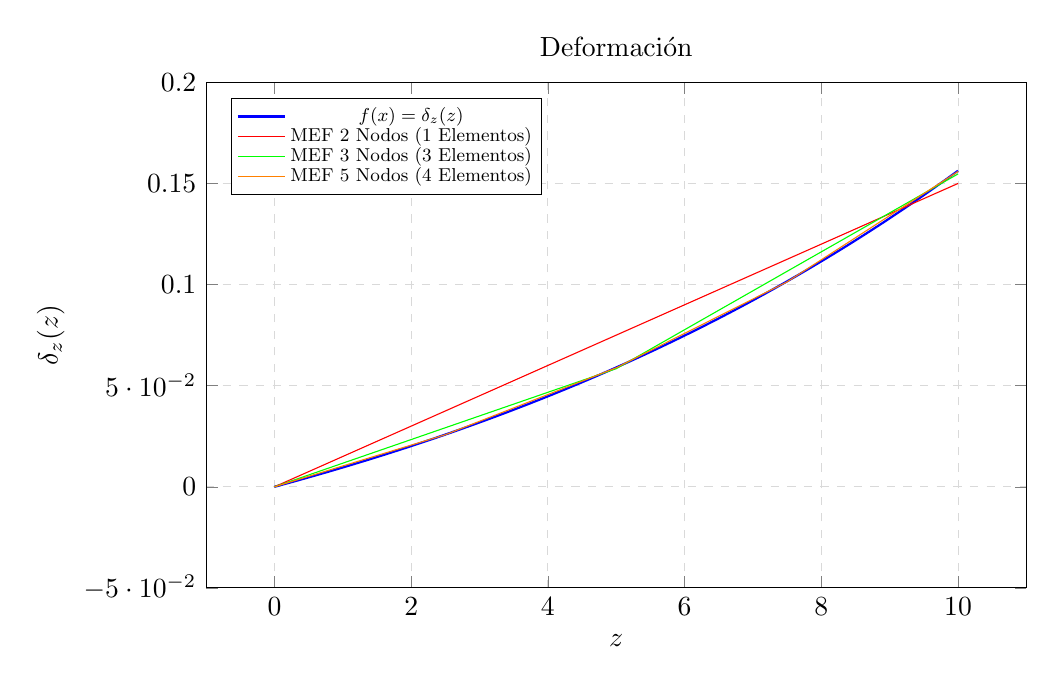
\begin{tikzpicture}
        \begin{axis}[
            title={Deformación},
            xlabel={$z$},
            ylabel={$\delta_z(z)$},
            grid=both, % Muestra la grilla
            grid style={dashed, gray!30},
            legend pos=north west, % Posición de la leyenda
            legend style={
    nodes={scale=0.75, transform shape}, % Escala todo el contenido al 75%
    font=\small,                         % Usa la fuente pequeña de LaTeX
    inner sep=2pt,                       % Reduce el relleno interior del recuadro
    row sep=-2pt                         % Junta un poco más las líneas de texto
},
            width=12cm,
            height=8cm,
            xmin=-1, xmax=11,
            ymin=-0.05, ymax=0.2
        ]
        
        % 1. Gráfica de la función continua
        \addplot [
            domain=0:10, 
            samples=100, % Cantidad de puntos para suavizar la curva
            color=blue,
            thick
        ]
        {3000*10000*(exp(x/10)-1)/(206000*1600)};
        \addlegendentry{$f(x) = \delta_z(z)$}
        

        
        \addplot [
            %%only marks, % Solo muestra los puntos, sin conectarlos con líneas
            mark=none, % Estilo del punto (círculo sólido)
            color=red,
            mark size=2.5pt
        ]
        coordinates {
            (0.0000, 0.00000)
            (10.0000, 0.15007)
        };
        \addlegendentry{MEF 2 Nodos (1 Elementos)}
        
        \addplot [
            %%only marks, % Solo muestra los puntos, sin conectarlos con líneas
            mark=none, % Estilo del punto (círculo sólido)
            color=green,
            mark size=2.5pt
        ]
            coordinates {
        (0.0000, 0.00000)
        (5.0000, 0.05844)
        (10.0000, 0.15478)
    };

        \addlegendentry{MEF 3 Nodos (3 Elementos)}

        
        \addplot [
           % %only marks, % Solo muestra los puntos, sin conectarlos con líneas
            mark=none, % Estilo del punto (círculo sólido)
            color=orange,
            mark size=2.5pt
        ]
            coordinates {
    (0.0000, 0.00000)
    (2.5000, 0.02578)
    (5.0000, 0.05889)
    (7.5000, 0.10140)
    (10.0000, 0.15599)
};


        \addlegendentry{MEF 5 Nodos (4 Elementos)}

                % 2. Gráfica del set de puntos (dispersión)
                % 2. Gráfica del set de puntos (dispersión)
%        \add¿plot [
            %%only marks, % Solo muestra los puntos, sin conectarlos con líneas
%            mark=none, % Estilo del punto (círculo sólido)
%            color=black,
%            mark size=2.5pt
%        ]
%        coordinates {
%    (0.0000, 0.00000)
%    (1.1111, 0.01069)
%    (2.2222, 0.02264)
%    (3.3333, 0.03599)
%    (4.4444, 0.05091)
%    (5.5556, 0.06758)
%    (6.6667, 0.08622)
%    (7.7778, 0.10704)
%    (8.8889, 0.13031)
%    (10.0000, 0.15632)
%};
%        \addlegendentry{MEF 10 Nodos}

        
        
        \end{axis}
    \end{tikzpicture}
\end{center}

Entonces ahora vamos a ver la diferencia de como se ven el ultimo nodos en todas las simulaciones MEF
\begin{center}  
    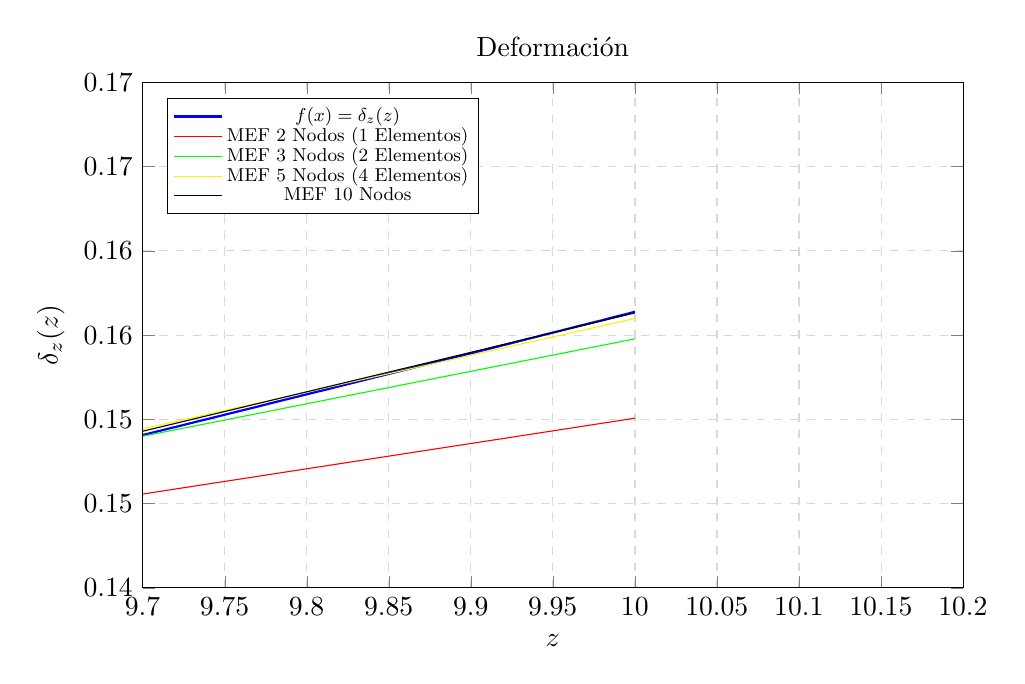
\begin{tikzpicture}
        \begin{axis}[
            title={Deformación},
            xlabel={$z$},
            ylabel={$\delta_z(z)$},
            grid=both, % Muestra la grilla
            grid style={dashed, gray!30},
            legend pos=north west, % Posición de la leyenda
            legend style={
    nodes={scale=0.75, transform shape}, % Escala todo el contenido al 75%
    font=\small,                         % Usa la fuente pequeña de LaTeX
    inner sep=2pt,                       % Reduce el relleno interior del recuadro
    row sep=-2pt                         % Junta un poco más las líneas de texto
},
            width=12cm,
            height=8cm,
            xmin=9.7, xmax=10.2,
            ymin=0.14, ymax=0.17
        ]
        
        % 1. Gráfica de la función continua
        \addplot [
            domain=9.5:10, 
            samples=100, % Cantidad de puntos para suavizar la curva
            color=blue,
            thick
        ]
        {3000*10000*(exp(x/10)-1)/(206000*1600)};
        \addlegendentry{$f(x) = \delta_z(z)$}
        

        
        \addplot [
            %only marks, % Solo muestra los puntos, sin conectarlos con líneas
            mark=none, % Estilo del punto (círculo sólido)
            color=red,
            mark size=2.5pt
        ]
        coordinates {
            (0.0000, 0.00000)
            (10.0000, 0.15007)
        };
        \addlegendentry{MEF 2 Nodos (1 Elementos)}
        
        \addplot [
            %only marks, % Solo muestra los puntos, sin conectarlos con líneas
            mark=none, % Estilo del punto (círculo sólido)
            color=green,
            mark size=2.5pt
        ]
            coordinates {
        (0.0000, 0.00000)
        (5.0000, 0.05844)
        (10.0000, 0.15478)
    };

        \addlegendentry{MEF 3 Nodos (2
        Elementos)}

        
        \addplot [
            %only marks, % Solo muestra los puntos, sin conectarlos con líneas
            mark=none, % Estilo del punto (círculo sólido)
            color=yellow,
            mark size=2.5pt
        ]
            coordinates {
    (0.0000, 0.00000)
    (2.5000, 0.02578)
    (5.0000, 0.05889)
    (7.5000, 0.10140)
    (10.0000, 0.15599)
};


        \addlegendentry{MEF 5 Nodos (4 Elementos)}

                % 2. Gráfica del set de puntos (dispersión)
        \addplot [
            %only marks, % Solo muestra los puntos, sin conectarlos con líneas
            mark=none, % Estilo del punto (círculo sólido)
            color=black,
            mark size=2.5pt
        ]
        coordinates {
    (0.0000, 0.00000)
    (1.1111, 0.01069)
    (2.2222, 0.02264)
    (3.3333, 0.03599)
    (4.4444, 0.05091)
    (5.5556, 0.06758)
    (6.6667, 0.08622)
    (7.7778, 0.10704)
    (8.8889, 0.13031)
    (10.0000, 0.15632)
};
        \addlegendentry{MEF 10 Nodos}

        
        
        \end{axis}
    \end{tikzpicture}
\end{center}
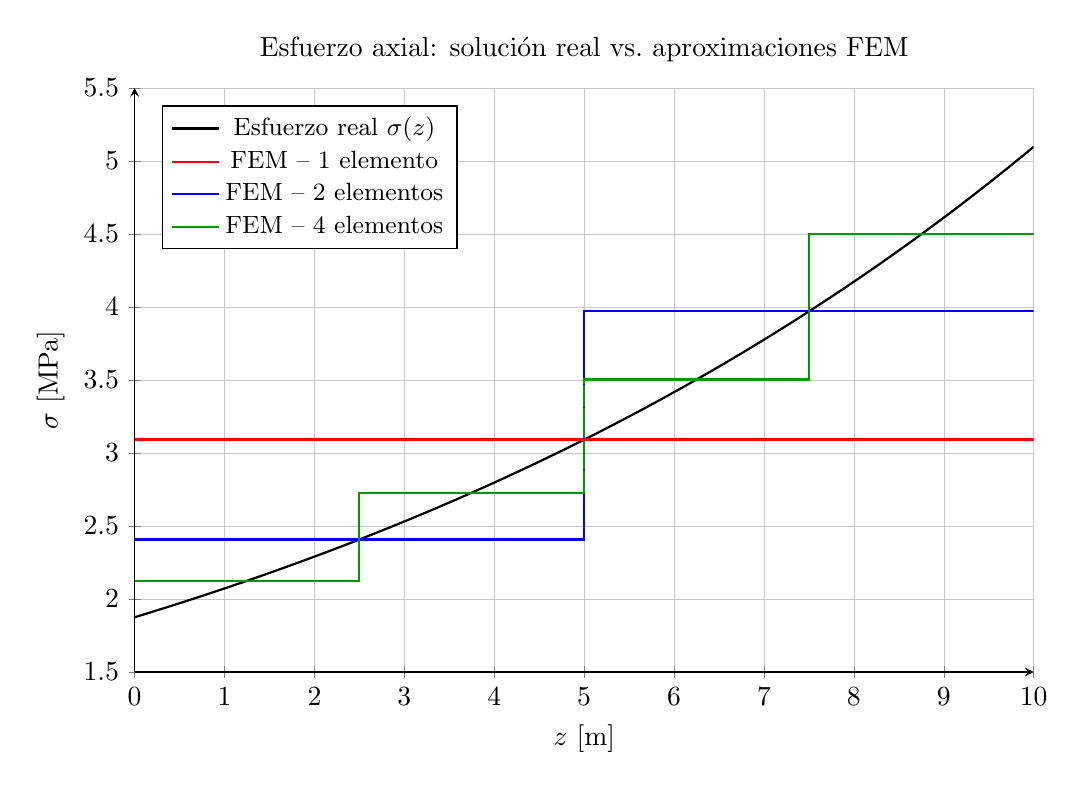
\begin{tikzpicture}
\begin{axis}[
    width=13cm, height=9cm,
    xlabel={$z$ [m]},
    ylabel={$\sigma$ [MPa]},
    title={Esfuerzo axial: solución real vs.\ aproximaciones FEM},
    xmin=0, xmax=10,
    ymin=1.5, ymax=5.5,
    grid=both,
    grid style={line width=.1pt, draw=gray!25},
    major grid style={line width=.2pt, draw=gray!45},
    legend pos=north west,
    legend style={font=\small},
    axis lines=left,
]
 
% --- Esfuerzo real (analitico): sigma(z) = 1.875 * exp(z/10) ---
\addplot[
    domain=0:10, samples=200,
    thick, black,
] {1.875*exp(x/10)};
\addlegendentry{Esfuerzo real $\sigma(z)$}
 
% --- 1 elemento (función escalón) ---
\addplot[
    const plot, thick, red, mark=none,
] coordinates {
    (0, 3.0914)
    (10, 3.0914)
};
\addlegendentry{FEM -- 1 elemento}
 
% --- 2 elementos (función escalón) ---
\addplot[
    const plot, thick, blue, mark=none,
] coordinates {
    (0, 2.4075)
    (5, 3.9694)
    (10, 3.9694)
};
\addlegendentry{FEM -- 2 elementos}
 
% --- 4 elementos (función escalón) ---
\addplot[
    const plot, thick, green!60!black, mark=none,
] coordinates {
    (0, 2.1247)
    (2.5, 2.7281)
    (5, 3.5030)
    (7.5, 4.4979)
    (10, 4.4979)
};
\addlegendentry{FEM -- 4 elementos}
 
% --- líneas punteadas verticales en los saltos (2 elementos) ---
\draw[blue, dotted, thick] (axis cs:5,2.4075) -- (axis cs:5,3.9694);
 
% --- líneas punteadas verticales en los saltos (4 elementos) ---
\draw[green!60!black, dotted, thick] (axis cs:2.5,2.1247) -- (axis cs:2.5,2.7281);
\draw[green!60!black, dotted, thick] (axis cs:5,2.7281)   -- (axis cs:5,3.5030);
\draw[green!60!black, dotted, thick] (axis cs:7.5,3.5030) -- (axis cs:7.5,4.4979);
 
\end{axis}
\end{tikzpicture}
Como podemos ver a medida que vamos aumentando la resolucion o la cantidad de nodos, de esta misma manera la cantidad de elementos el resultado se hace cada vez mas parecido al real
\end{desarrollo}


\newpage
 \section*{Problema 2}
 
Se propone diseñar una estructura reticulada plana formada por barras de acero
($E = 206$ GPa y $S_y = 300$ MPa) que cubra una longitud determinada
($L = 20$ m) y que sea capaz de soportar la acción de una fuerza vertical
situada en el centro de la luz ($P = 50$ kN). Las barras a utilizar (el número
de barras a considerar en el diseño es de libre elección) tienen sección
transversal constante ($A = 1000$ mm$^2$) y una longitud máxima dada
($L_{\text{max-barra}} = 5$ m). Despreciar en el cálculo por MEF el peso
propio de las barras. Como restricción de diseño, se pide que la tensión en
ninguna de las barras supere el límite elástico y que la deflexión máxima sea
menor a un valor dado ($v_{\max} = 10$ mm). Se piden al menos dos diseños
distintos, analizando sus ventajas y desventajas. Adicionalmente, se pide
extender a tres dimensiones uno de los diseños anteriores.
 
\bigskip
 
\begin{center}
\begin{tikzpicture}[scale=1, every node/.style={font=\normalsize}]
 
    % --- Datos geometricos ---
    \def\Ltot{8}     % longitud total representada en el dibujo
    \def\yBeam{0}    % altura de la linea de la luz
 
    % --- Linea de la luz (span) ---
    \draw[thick] (0,\yBeam) -- (\Ltot,\yBeam);
 
    % --- Apoyos fijos (empotramientos triangulares con rayado) ---
    \foreach \x in {0,\Ltot} {
        \draw[thick] (\x,0) -- (\x-0.35,-0.6) -- (\x+0.35,-0.6) -- cycle;
        \foreach \i in {-0.3,-0.15,...,0.3} {
            \draw[thick] (\x+\i,-0.6) -- (\x+\i-0.15,-0.85);
        }
    }
 
    % --- Cota L/2 (mas cercana a la viga) ---
    \draw[{Latex[length=2mm]}-{Latex[length=2mm]}] (0,0.5) -- (\Ltot/2,0.5);
    \draw[thin] (0,0.35) -- (0,0.65);
    \draw[thin] (\Ltot/2,0.35) -- (\Ltot/2,0.65);
    \node at (\Ltot/4,0.8) {$L/2$};
 
    % --- Cota L (por encima de L/2) ---
    \draw[{Latex[length=2mm]}-{Latex[length=2mm]}] (0,1.3) -- (\Ltot,1.3);
    \draw[thin] (0,1.15) -- (0,1.45);
    \draw[thin] (\Ltot,1.15) -- (\Ltot,1.45);
    \node at (\Ltot/2-0.4,1.6) {$L$};
 
    % --- Fuerza P en el centro (por encima de ambas cotas) ---
    \draw[-{Latex[length=3mm]}, thick] (\Ltot/2,2.6) -- (\Ltot/2,1.75);
    \node at (\Ltot/2+0.3,2.45) {$P$};
 
\end{tikzpicture}
\end{center}

\begin{desarrollo}{Problema 2 Desarrollo teorico del problema}
    Ahora el problema se complejiza un poco mas, para poder iniciar, lo clave es saber cuales son los datos que tengo que tener y cuales tengo que sacar (input/output).
    Para mi caso y todosa los codigos utilice una libreria de python llamada \textit{pint} la cual me permite cambiar facilemente entre unidades y despreocuparme de ese ámbito.(explicare el codigo para 3D pero es lo mismo para 2D sin z)\\

    \textbf{Paso 1: Inputs}\\
    Los nodos en este caso no estan todos en una misma linea recta, equidistante. Por ende necesito una lista de puntos los cuales me muestre donde va cada nodo, no es necesario numerarlos ya que la misma lista los enumera, pero cada nodo tiene sus coordenadas respectivas (3D:$[x,y,z]$), otro es que nodo conecto con cual nodo, para esto utilizo la matriz de conectividad que es una lista que contiene nodo 1 nodo 2, asi conecto 1 y 2 (para la limitante de longitud 5 solo tuve un print que me avisaba), luego tengo los apoyos, esto tienen una lista que tiene $[\text{nodo}, r_x,r_y,r_z]$ y finalmente las fuerzas, en mi caso al no tener fuerzas distribuidas no tuve que lidiar el problema de que nodo se lleva cuanta fuerza pero para las fuerzas externas ($P=50\textbf{kN}$) tengo una matriz que toma 
    $[\text{Nodo},f_x,f_y,f_z]$\\

    \textbf{Paso 2: Matriz de rigidez}\\
    Todo esto se basa en que los inputs de los elementos solo admiten fuerzas axiales, por ende tomamos la matriz de rigidez local (la que le hace a la barra verse como el centro del mundo) y la pasamos por la matriz de rotacion.
    Ahora esta matriz de rotación no es nada mas que una matriz de proyección ortogonal ($T= U(U^T U)^{-1}U^T$)
    Donde $U$ es el vector posición de la barra (Podria no usar la parte de $(U^T U)^{-1}$ pero se encarga de normalizar, básicamente asegurarme que esta matriz no escale nada, determinante 1)pero para la matriz real de transformación tengo que tener en cuenta los dos nodos.\\
    
Como $T$ ya es una proyección expresada en coordenadas globales (no locales), no necesito pasar por una rotación intermedia: la fuerza axial en cada nodo depende solo de la componente de $U$ proyectada sobre la dirección de la barra. Para el nodo $n$:
$$F_n = \frac{EA}{L}\,T\,(U_n - U_m)$$
y por equilibrio, $F_m = -F_n = \dfrac{EA}{L}\,T\,(U_m - U_n)$. Matricialmente:
$$\begin{bmatrix} F_n\\ F_m \end{bmatrix} = \frac{EA}{L}\begin{bmatrix} T & -T\\ -T & T \end{bmatrix}\begin{bmatrix} U_n\\ U_m \end{bmatrix} = K_e \begin{bmatrix} U_n\\ U_m \end{bmatrix}$$
Es decir, la matriz de rigidez del elemento, ya expresada en coordenadas globales, es directamente
$$K_e = \frac{EA}{L}\begin{bmatrix} T & -T\\ -T & T \end{bmatrix}$$

\textbf{Paso 3: Ensamble de la matriz general}\\
La matriz global $K$ tiene tamaño $(N\cdot d)\times(N\cdot d)$, donde $N$ es el número total de nodos y $d$ los grados de libertad por nodo ($d=2$ en 2D, $d=3$ en 3D). Cada nodo $k$ ocupa el bloque de filas y columnas $[kd:(k+1)d]$ dentro de $K$.

Para cada elemento que conecta los nodos $n$ y $m$, tomo los cuatro bloques de $K_e$ obtenidos antes y los sumo en las posiciones correspondientes de $K$:
$$K[n,n] \mathrel{+}= K_{nn}, \qquad K[n,m] \mathrel{+}= K_{nm}, \qquad K[m,n] \mathrel{+}= K_{mn}, \qquad K[m,m] \mathrel{+}= K_{mm}$$
donde $K_{nn}=K_{mm}=\dfrac{EA}{L}T$ y $K_{nm}=K_{mn}=-\dfrac{EA}{L}T$.\\

\begin{lstlisting}[style=pythonstyle, caption={Ensamblaje de la matriz de rigidez global}, label={lst:gen_matriz_global}]
## Generadora de la matriz
def gen_matriz_global(xyz, conectividad, Area, M_Elasticidad=206*ureg.GPa):
    num_nodos = len(xyz)
    num_elementos = len(conectividad)
    dim = xyz.shape[1]          
    n_lib = num_nodos * dim     

    K_global = np.zeros((n_lib, n_lib)) * (ureg.newton / ureg.meter)# creo aqui la matriz general

    for e in range(num_elementos):
        n1, n2 = conectividad[e]
        p1 = xyz[n1] #en vez de trabajar con cada uno separado trabajo todos como 1 punto
        p2 = xyz[n2]
        delta = (p2 - p1).to(ureg.meter)        #Esos son los deltas de los componentes
        L_e = np.sqrt(np.sum(delta**2))
        n_dir = (delta / L_e).magnitude         # vector de cosenos directores [cx,cy] o [cx,cy,cz]
        k_const = (M_Elasticidad * Area / L_e).to(ureg.newton / ureg.meter)
        # Para este caso lo que tenemos que hacer es la proyeccion ortogonal, por ende matricialmente applicamos T= U(U^T U)^-1U^T
        T = np.outer(n_dir, n_dir)              #Eso se puede hacer con el producto externo que me genera la matriz de proyeccion pero eso es para 1 nodo, y necesito para 2
        ke_sub = np.block([[ T, -T],
                            [-T,  T]])           # Aqui se lo aplico a cada uno de los nodos
        ke_global = k_const * ke_sub
        # Lo mismo que en 2D, pero ahora tengo en cuenta 3  o 2 o 1 dimensiones.
        dofs = [dim*n1 + k for k in range(dim)] + [dim*n2 + k for k in range(dim)] #suma de dos listas, la primera es para el nodo 1 y la segunda para el nodo 2, y cada una tiene los grados de libertad de cada nodo

        for i in range(2*dim):
            for j in range(2*dim):
                K_global[dofs[i], dofs[j]] += ke_global[i, j]

    return K_global
\end{lstlisting}
\textbf{Paso 4: aplicacion de cargas y restricciones}\\
Para este caso se tiene que las cargas son simplemente cambiar el vectore de fuerzas externas, ya que todas las fueras internas deben ser iguales a las externas ($\textbf{KU}=\textbf{F}$), para esto solo coloco las fuerzas en los nodos del medio. Dependiendo del puente veo si se puede colocar exactamente en el medio o veo si no, entonces lo coloco dividido equitativamente (generalmente intento que quede simétrico por eso equitativamente) entre los nodos del medio.
Para las restricciones tengo 2 opciones, como se que la restriccion es que $u_{n1}=0$ entinces esa ecuacion la elimino y coloco una que multiplicada por ese vector me da 0, que seria basicamente mantener tamaño de matriz pero cambiar ecuaciones para resolver el sistema. mejor y mas facil es crear una matriz $K_{red}$ la cual es igual pero donde haya una restriccion elimino columna y fila correspondiente, asi se mantiene cuadrada, tambien tengo que eliminar esos mismos elementos de $U$ y de $F$, de esta manera obtengo 3 cosas reducidad, matriz de rigidez, vector de fuerzas, y vector de desplazamientos reducido.\\
\begin{lstlisting}[style=pythonstyle, caption={Ensamblaje del vector de fuerzas global}, label={lst:gen_f_global}]
#el vector de fuerzas 
def gen_f_global(xyz, f_nodales):
    dim = xyz.shape[1]
    n_lib = len(xyz) * dim
    F_global = np.zeros(n_lib) * ureg.newton
    for entrada in f_nodales:
        nodo = entrada[0]
        fuerzas = entrada[1:]            # (fx,fy) o (fx,fy,fz)
        for k, f in enumerate(fuerzas):
            F_global[dim*nodo + k] += f
    return F_global
\end{lstlisting}

\begin{lstlisting}[style=pythonstyle, caption={Determinación de los grados de libertad restringidos}, label={lst:restricciones}]
##Aqui hago loa apoyos
def Restriciones(apoyos):
    dim = apoyos.shape[1] - 1         # Resto 1 por el numero del nodo en cual esta
    dofs_fijos = []
    for entrada in apoyos:
        nodo = entrada[0]
        restricciones = entrada[1:]
        for k, r in enumerate(restricciones):
            if r == 1:
                dofs_fijos.append(dim*nodo + k)
    return sorted(dofs_fijos)
\end{lstlisting}

\textbf{Paso 5: Resolución del sistema}\\
Para resolverlo, es bastante facil, aplico en python 
$$Ax=b$$ y resuelvo. de esta manera obtengo los desplazamientos nodales, de cada nodo.\\
\begin{lstlisting}[style=pythonstyle, caption={Reducción del sistema y resolución de desplazamientos}, label={lst:sis_reducido}]
#no hay cambias como es redicr las que tienen restricciones y resolver
def Sis_reducido(K_global, F_global, dofs_fijos):
    K_reducida = np.delete(np.delete(K_global, dofs_fijos, axis=0), dofs_fijos, axis=1)
    F_reducida = np.delete(F_global, dofs_fijos, axis=0)
    U_red = np.linalg.solve(K_reducida, F_reducida)
    return U_red, K_reducida, F_reducida
\end{lstlisting}
\textbf{Paso 6: Desplazamientos nodales}\\
Para este caso lo que tenemos que hacer es agregar los desplazamientos que habimos restringido, (que son 0) y esto lo hacemos en orden, previamente se guardo un vector que decia los nodos que estaban restringidos, y ahora en esas posiciones colocamos 0, en el resto los valores de $U_{red}$ en orden.\\
\begin{lstlisting}[style=pythonstyle, caption={Reconstrucción del vector de desplazamientos completo}, label={lst:u_completa}]
#aqui lleno el resto de las filas
def U_completa(dofs_fijos, U_red):
    n_lib = len(U_red) + len(dofs_fijos)
    gl_libres = [d for d in range(n_lib) if d not in dofs_fijos]
    U = np.zeros(n_lib) * U_red.units
    U[gl_libres] = U_red
    return U
\end{lstlisting}
\textbf{Paso 7: Calculo de esfuerzos}\\
Para este caso, en lugar de calcular las posiciones desplazadas exactas, el cambio de longitud se obtiene proyectando el desplazamiento relativo de los nodos sobre la dirección original de la barra. Esto se logra de forma mucho más directa mediante un producto punto, lo cual es la formulación estándar bajo el supuesto de pequeños desplazamientos.

Primero, se determina la longitud inicial de la barra y su vector unitario direccional $\hat{n}$, el cual indica la orientación de la barra en el espacio tridimensional:
$$\ell_0 = \sqrt{dx_0^2 + dy_0^2 + dz_0^2}$$
$$\hat{n} = \left( \dfrac{dx_0}{\ell_0}, \dfrac{dy_0}{\ell_0}, \dfrac{dz_0}{\ell_0} \right)$$

A continuación, se define el vector de desplazamiento relativo $\Delta \vec{u}$, que representa la diferencia de movimiento entre el nodo final (2) y el nodo inicial (1):
$$\Delta \vec{u} = \left( u_{2x} - u_{1x}, u_{2y} - u_{1y}, u_{2z} - u_{1z} \right)$$

El cambio de longitud de la barra ($\Delta \ell$) corresponde simplemente al producto punto entre el vector de desplazamiento relativo y el vector unitario de la barra. Esta operación extrae únicamente la componente del desplazamiento que alarga o acorta el elemento:
$$\Delta \ell = \Delta \vec{u} \cdot \hat{n}$$

Con esto, la deformación unitaria se calcula dividiendo esta elongación por la longitud original:
$$\varepsilon = \dfrac{\Delta \ell}{\ell_0}$$

Ahora, aplicando la relación constitutiva del material (Ley de Hooke), el esfuerzo normal se obtiene como:
$$\sigma = E\varepsilon$$

En caso de requerir la fuerza interna axial que soporta el elemento, basta con multiplicar el esfuerzo obtenido por el área de la sección transversal $A$:
$$F = \sigma \cdot A$$

\begin{lstlisting}[style=pythonstyle, caption={Cálculo de fuerza axial y esfuerzo por elemento}, label={lst:calc_esfuerzos}]
#Fuerza axial y esfuerzo en cada elemento, misma logica que gen_matriz_global
#pero ahora en vez de armar la matriz, proyecto el desplazamiento relativo
#(u2-u1) sobre la direccion de la barra para sacar el alargamiento
def calc_esfuerzos(xyz, conectividad, U, Area, M_Elasticidad=206*ureg.GPa):
    dim = xyz.shape[1]
    num_elementos = len(conectividad)
    fuerzas = np.zeros(num_elementos) * ureg.newton
    esfuerzos = np.zeros(num_elementos) * ureg.MPa

    for e in range(num_elementos):
        n1, n2 = conectividad[e]
        p1, p2 = xyz[n1], xyz[n2]

        delta = (p2 - p1).to(ureg.meter)
        L_e = np.sqrt(np.sum(delta**2))
        n_dir = (delta / L_e).magnitude          # mismo vector de cosenos directores

        u1 = U[dim*n1:dim*n1+dim].to(ureg.meter).magnitude
        u2 = U[dim*n2:dim*n2+dim].to(ureg.meter).magnitude
        elongacion = np.dot(n_dir, u2 - u1) * ureg.meter   # positivo = se alarga (traccion)

        k_const = (M_Elasticidad * Area / L_e).to(ureg.newton / ureg.meter)
        N = (k_const * elongacion).to(ureg.newton)

        fuerzas[e] = N
        esfuerzos[e] = (N / Area).to(ureg.MPa)

    return fuerzas, esfuerzos
\end{lstlisting}
\end{desarrollo}





\begin{desarrollo}{Propuesta 1 de Puente}
    

Este fue en problema de estatica por ende reutilice la matriz de nodos y conectividad, tuve que cambiar escala para poder que cumpla.
\begin{center}
\begin{tikzpicture}[scale=0.5]
\tikzset{joint/.style={circle, fill=black, inner sep=1.5pt}}
% Nodos (coordenadas en metros)
\coordinate (n0)  at (0,0);
\coordinate (n1)  at (2,0);
\coordinate (n2)  at (2,1);
\coordinate (n3)  at (4,0);
\coordinate (n4)  at (4,2);
\coordinate (n5)  at (6,0);
\coordinate (n6)  at (6,2.75);
\coordinate (n7)  at (8,0);
\coordinate (n8)  at (8,3.25);
\coordinate (n9)  at (10,0);
\coordinate (n10) at (10,3.5);
\coordinate (n11) at (12,0);
\coordinate (n12) at (12,3.25);
\coordinate (n13) at (14,0);
\coordinate (n14) at (14,2.75);
\coordinate (n15) at (16,0);
\coordinate (n16) at (16,2);
\coordinate (n17) at (18,0);
\coordinate (n18) at (18,1);
\coordinate (n19) at (20,0);
% Elementos (barras)
\draw[thick]
  (n0)--(n1)  (n0)--(n2)  (n1)--(n2)  (n1)--(n3)  (n2)--(n3)
  (n2)--(n4)  (n3)--(n4)  (n3)--(n5)  (n3)--(n6)  (n4)--(n6)
  (n5)--(n6)  (n5)--(n7)  (n6)--(n7)  (n6)--(n8)  (n7)--(n8)
  (n7)--(n9)  (n7)--(n10) (n8)--(n10) (n9)--(n10) (n9)--(n11)
  (n10)--(n11)(n10)--(n12)(n11)--(n12)(n11)--(n13)(n11)--(n14)
  (n12)--(n14)(n13)--(n14)(n13)--(n15)(n14)--(n15)(n14)--(n16)
  (n15)--(n16)(n15)--(n17)(n15)--(n18)(n16)--(n18)(n17)--(n18)
  (n17)--(n19)(n18)--(n19);
% Nodos (puntos)
\foreach \n in {0,...,19}{\node[joint] at (n\n) {};}
% Etiquetas de nodo
\foreach \n in {0,1,3,5,7,9,11,13,15,17,19}{\node[below=2pt] at (n\n) {\tiny \n};}
\foreach \n in {2,4,6,8,10,12,14,16,18}{\node[above=2pt] at (n\n) {\tiny \n};}
% Apoyo fijo en nodo 0 (rx=1, ry=1)
\draw[fill=gray!40] (0,0) -- (-0.4,-0.7) -- (0.4,-0.7) -- cycle;
\draw (-0.6,-0.7) -- (0.6,-0.7);
\foreach \x in {-0.6,-0.4,-0.2,0,0.2,0.4}{\draw (\x,-0.7) -- (\x-0.15,-0.95);}
% Apoyo fijo en nodo 19 (rx=1, ry=1)
\draw[fill=gray!40] (20,0) -- (19.6,-0.7) -- (20.4,-0.7) -- cycle;
\draw (19.4,-0.7) -- (20.6,-0.7);
\foreach \x in {19.4,19.6,19.8,20.0,20.2,20.4}{\draw (\x,-0.7) -- (\x-0.15,-0.95);}
% Fuerzas nodales
\draw[-{Latex[length=3mm]}, thick, red] (n9) -- ++(0,-1.5) node[below] {\small $50\,\text{kN}$};

% ===== COTAS =====
% Luz total: 20 m (abajo del todo, bajo la etiqueta de la fuerza)
\draw[thin] (0,-0.95) -- (0,-2.3);
\draw[thin] (20,-0.95) -- (20,-2.3);
\draw[{Latex[length=2mm]}-{Latex[length=2mm]}, thin] (0,-2.3) -- (20,-2.3)
  node[midway, below] {\small $20\text{ m}$};

% Altura máxima: 3.5 m (junto al nodo 10)
\draw[dashed, thin] (-1,0) -- (10,0);
\draw[dashed,thin] (-1,3.5) -- (10,3.5);
\draw[{|Latex[length=2mm]}-{Latex[length=2mm]|}, thin] (-1,0) -- (-1,3.5)
  node[midway, right] {\small $3.5\text{ m}$};
\end{tikzpicture}

\end{center}


Como podemos apreciar ninguna barra tiene un largo mayor a $5 \text{m}$, esto debido a que el largo mayor es $$\sqrt{2^2+3.5^2}=4.031\text{m}$$



% ===== MACRO: color proporcional al esfuerzo (generalizado) =====
\def\smax{51.00}   % maximo esfuerzo de traccion (MPa)
\def\smin{63.41717}   % magnitud del minimo esfuerzo de compresion (MPa)

\begin{center}
\begin{tikzpicture}[scale=0.5]
\tikzset{joint/.style={circle, fill=black, inner sep=1.5pt}}
% Nodos (coordenadas en metros)
\coordinate (n0)  at (0,0);
\coordinate (n1)  at (2,0);
\coordinate (n2)  at (2,1);
\coordinate (n3)  at (4,0);
\coordinate (n4)  at (4,2);
\coordinate (n5)  at (6,0);
\coordinate (n6)  at (6,2.75);
\coordinate (n7)  at (8,0);
\coordinate (n8)  at (8,3.25);
\coordinate (n9)  at (10,0);
\coordinate (n10) at (10,3.5);
\coordinate (n11) at (12,0);
\coordinate (n12) at (12,3.25);
\coordinate (n13) at (14,0);
\coordinate (n14) at (14,2.75);
\coordinate (n15) at (16,0);
\coordinate (n16) at (16,2);
\coordinate (n17) at (18,0);
\coordinate (n18) at (18,1);
\coordinate (n19) at (20,0);

% ===== BARRAS con color proporcional al esfuerzo exacto =====
\sigmabar{n0}{n1}{-5.853638925271909}
\sigmabar{n0}{n2}{-55.6930643466406}
\sigmabar{n1}{n2}{0.0909262446970871}
\sigmabar{n1}{n3}{-6.001135102121191}
\sigmabar{n2}{n3}{0.10275795691206817}
\sigmabar{n2}{n4}{-55.8302436489914}
\sigmabar{n3}{n4}{6.292775591215882}
\sigmabar{n3}{n5}{-1.5358251934491918}
\sigmabar{n3}{n6}{-7.710196597470205}
\sigmabar{n4}{n6}{-53.383397147216115}
\sigmabar{n5}{n6}{0.016088728940776387}
\sigmabar{n5}{n7}{-1.5303691712977852}
\sigmabar{n6}{n7}{11.909582408226585}
\sigmabar{n6}{n8}{-63.41717007402167}
\sigmabar{n7}{n8}{7.6967946797469065}
\sigmabar{n7}{n9}{15.373981268426817}
\sigmabar{n7}{n10}{-19.93316839154642}
\sigmabar{n8}{n10}{-62.00}
\sigmabar{n9}{n10}{50.00}
\sigmabar{n9}{n11}{15.373981268335335}
\sigmabar{n10}{n11}{-19.93316839159181}
\sigmabar{n10}{n12}{-62.00869063353391}
\sigmabar{n11}{n12}{7.6967946797469065}
\sigmabar{n11}{n13}{-1.5303691711148204}
\sigmabar{n11}{n14}{11.909582408307296}
\sigmabar{n12}{n14}{-63.41717007393294}
\sigmabar{n13}{n14}{0.016088728940776387}
\sigmabar{n13}{n15}{-1.535825193723639}
\sigmabar{n14}{n15}{-7.710196597550915}
\sigmabar{n14}{n16}{-53.38339714734461}
\sigmabar{n15}{n16}{6.292775591215882}
\sigmabar{n15}{n17}{-6.001135101846744}
\sigmabar{n15}{n18}{0.10275795711662898}
\sigmabar{n16}{n18}{-55.83024364882774}
\sigmabar{n17}{n18}{0.0909262446970871}
\sigmabar{n17}{n19}{-5.853638925363391}
\sigmabar{n18}{n19}{-55.69306434668151}

% Nodos
\foreach \n in {0,...,19}{\node[joint] at (n\n) {};}
\foreach \n in {0,1,3,5,7,9,11,13,15,17,19}{\node[below=2pt] at (n\n) {\tiny \n};}
\foreach \n in {2,4,6,8,10,12,14,16,18}{\node[above=2pt] at (n\n) {\tiny \n};}

% Apoyos
\draw[fill=gray!40] (0,0) -- (-0.4,-0.7) -- (0.4,-0.7) -- cycle;
\draw (-0.6,-0.7) -- (0.6,-0.7);
\foreach \x in {-0.6,-0.4,-0.2,0,0.2,0.4}{\draw (\x,-0.7) -- (\x-0.15,-0.95);}
\draw[fill=gray!40] (20,0) -- (19.6,-0.7) -- (20.4,-0.7) -- cycle;
\draw (19.4,-0.7) -- (20.6,-0.7);
\foreach \x in {19.4,19.6,19.8,20.0,20.2,20.4}{\draw (\x,-0.7) -- (\x-0.15,-0.95);}

% Carga
\draw[-{Latex[length=3mm]}, thick, black] (n9) -- ++(0,-1.5) node[below] {\small $50\,\text{kN}$};
\end{tikzpicture}

\vspace{0.5em}
% ===== COLORBAR =====
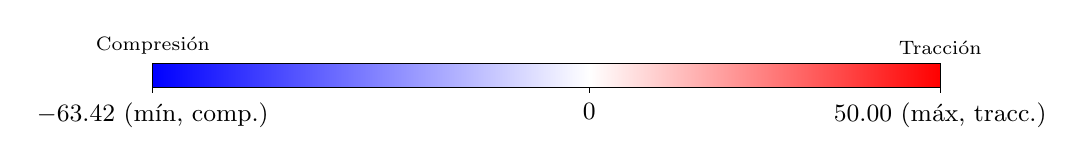
\begin{tikzpicture}[scale=0.5]
\def\barlen{20}
\def\barh{0.6}
\pgfmathsetmacro{\zeropos}{\barlen*\smin/(\smin+\smax)}
\shade[left color=blue, right color=white] (0,0) rectangle (\zeropos,\barh);
\shade[left color=white, right color=red] (\zeropos,0) rectangle (\barlen,\barh);
\draw (0,0) rectangle (\barlen,\barh);
\draw (0,0) -- (0,-0.15) node[below] {\small $-63.42$ (mín, comp.)};
\draw (\zeropos,0) -- (\zeropos,-0.15) node[below] {\small $0$};
\draw (\barlen,0) -- (\barlen,-0.15) node[below] {\small $50.00$ (máx, tracc.)};
\node[above] at (0,\barh) {\scriptsize Compresión};
\node[above] at (\barlen,\barh) {\scriptsize Tracción};
\end{tikzpicture}
\end{center}




% ===== FACTOR DE AMPLIFICACION =====
\def\amp{100} % ajusta este valor si la deformada se ve muy chica o muy exagerada

% Calcula coordenada deformada: (x0,y0) + amp*(ux,uy)[mm->m]

\begin{center}
\begin{tikzpicture}[scale=0.5]
\tikzset{joint/.style={circle, fill=black, inner sep=1.5pt}}
\tikzset{jointdef/.style={circle, fill=red!70!black, inner sep=1.3pt}}

% ===== Nodos originales =====
\coordinate (n0)  at (0,0);
\coordinate (n1)  at (2,0);
\coordinate (n2)  at (2,1);
\coordinate (n3)  at (4,0);
\coordinate (n4)  at (4,2);
\coordinate (n5)  at (6,0);
\coordinate (n6)  at (6,2.75);
\coordinate (n7)  at (8,0);
\coordinate (n8)  at (8,3.25);
\coordinate (n9)  at (10,0);
\coordinate (n10) at (10,3.5);
\coordinate (n11) at (12,0);
\coordinate (n12) at (12,3.25);
\coordinate (n13) at (14,0);
\coordinate (n14) at (14,2.75);
\coordinate (n15) at (16,0);
\coordinate (n16) at (16,2);
\coordinate (n17) at (18,0);
\coordinate (n18) at (18,1);
\coordinate (n19) at (20,0);

% ===== Nodos deformados (original + amp * desplazamiento) =====
\dnode{m0}{0}{0}{0}{0}
\dnode{m1}{2}{0}{-0.05926112722229112}{-3.117441790289405}
\dnode{m2}{2}{1}{0.8803022126508393}{-3.117441790289405}
\dnode{m3}{4}{0}{-0.11852225444458224}{-5.115090724480247}
\dnode{m4}{4}{2}{1.1703681914271549}{-5.0544111128297615}
\dnode{m5}{6}{0}{-0.13365275501197516}{-6.0522667159018715}
\dnode{m6}{6}{2.75}{0.953210628015924}{-6.0522667159018715}
\dnode{m7}{8}{0}{-0.14878325557936836}{-7.096384343964715}
\dnode{m8}{8}{3.25}{0.5295612109511663}{-6.975025120663744}
\dnode{m9}{10}{0}{0}{-8.480196688089908}
\dnode{m10}{10}{3.5}{0}{-7.630682124983113}
\dnode{m11}{12}{0}{0.14878325557937458}{-7.096384343964709}
\dnode{m12}{12}{3.25}{-0.5295612109511653}{-6.97502512066374}
\dnode{m13}{14}{0}{0.1336527550119805}{-6.0522667159018635}
\dnode{m14}{14}{2.75}{-0.953210628015922}{-6.0522667159018635}
\dnode{m15}{16}{0}{0.11852225444458649}{-5.115090724480236}
\dnode{m16}{16}{2}{-1.170368191427151}{-5.054411112829749}
\dnode{m17}{18}{0}{0.05926112722229323}{-3.1174417902893925}
\dnode{m18}{18}{1}{-0.880302212650835}{-3.1174417902893925}
\dnode{m19}{20}{0}{0}{0}

% ===== Estructura original (referencia, gris punteado) =====
\draw[dashed, gray, line width=0.8pt]
  (n0)--(n1)  (n0)--(n2)  (n1)--(n2)  (n1)--(n3)  (n2)--(n3)
  (n2)--(n4)  (n3)--(n4)  (n3)--(n5)  (n3)--(n6)  (n4)--(n6)
  (n5)--(n6)  (n5)--(n7)  (n6)--(n7)  (n6)--(n8)  (n7)--(n8)
  (n7)--(n9)  (n7)--(n10) (n8)--(n10) (n9)--(n10) (n9)--(n11)
  (n10)--(n11)(n10)--(n12)(n11)--(n12)(n11)--(n13)(n11)--(n14)
  (n12)--(n14)(n13)--(n14)(n13)--(n15)(n14)--(n15)(n14)--(n16)
  (n15)--(n16)(n15)--(n17)(n15)--(n18)(n16)--(n18)(n17)--(n18)
  (n17)--(n19)(n18)--(n19);

% ===== Estructura deformada (solida, coloreada) =====
\draw[thick, blue!70!black]
  (m0)--(m1)  (m0)--(m2)  (m1)--(m2)  (m1)--(m3)  (m2)--(m3)
  (m2)--(m4)  (m3)--(m4)  (m3)--(m5)  (m3)--(m6)  (m4)--(m6)
  (m5)--(m6)  (m5)--(m7)  (m6)--(m7)  (m6)--(m8)  (m7)--(m8)
  (m7)--(m9)  (m7)--(m10) (m8)--(m10) (m9)--(m10) (m9)--(m11)
  (m10)--(m11)(m10)--(m12)(m11)--(m12)(m11)--(m13)(m11)--(m14)
  (m12)--(m14)(m13)--(m14)(m13)--(m15)(m14)--(m15)(m14)--(m16)
  (m15)--(m16)(m15)--(m17)(m15)--(m18)(m16)--(m18)(m17)--(m18)
  (m17)--(m19)(m18)--(m19);

% Nodos originales (fantasma) y deformados
\foreach \n in {0,...,19}{\node[joint, fill=gray!60] at (n\n) {};}
\foreach \n in {0,...,19}{\node[jointdef] at (m\n) {};}

% Apoyos (en posicion original, no se mueven)
\draw[fill=gray!40] (0,0) -- (-0.4,-0.7) -- (0.4,-0.7) -- cycle;
\draw (-0.6,-0.7) -- (0.6,-0.7);
\foreach \x in {-0.6,-0.4,-0.2,0,0.2,0.4}{\draw (\x,-0.7) -- (\x-0.15,-0.95);}
\draw[fill=gray!40] (20,0) -- (19.6,-0.7) -- (20.4,-0.7) -- cycle;
\draw (19.4,-0.7) -- (20.6,-0.7);
\foreach \x in {19.4,19.6,19.8,20.0,20.2,20.4}{\draw (\x,-0.7) -- (\x-0.15,-0.95);}

% Etiqueta del desplazamiento maximo (nodo 9)
\draw[-{Latex[length=2mm]}, thin] (m9) -- ++(1.5,-0.3)
   node[right] {\small $u_{y,9} = -8.48\,\text{mm}$};
\end{tikzpicture}

\vspace{0.3em}
{\small
\tikz[baseline=-0.5ex]\draw[dashed, gray, line width=1pt] (0,0)--(0.5,0); \; Estructura original \qquad
\tikz[baseline=-0.5ex]\draw[thick, blue!70!black] (0,0)--(0.5,0); \; Deformada (amplificada $\times\,100$)
}
\end{center}

\end{desarrollo}




\begin{desarrollo}{Propuesta 2 de puente}
    
\begin{center}
\begin{tikzpicture}[scale=0.5]
\tikzset{joint/.style={circle, fill=black, inner sep=1.5pt}}
% Nodos (coordenadas en metros)
\coordinate (n0)  at (0,0);
\coordinate (n1)  at (4,0);
\coordinate (n2)  at (8,0);
\coordinate (n3)  at (12,0);
\coordinate (n4)  at (16,0);
\coordinate (n5)  at (20,0);
\coordinate (n6)  at (0,3);
\coordinate (n7)  at (4,3);
\coordinate (n8)  at (8,3);
\coordinate (n9)  at (12,3);
\coordinate (n10) at (16,3);
\coordinate (n11) at (20,3);
% Elementos (barras)
% Cuerda inferior
\draw[thick] (n0)--(n1)--(n2)--(n3)--(n4)--(n5);
% Cuerda superior
\draw[thick] (n6)--(n7)--(n8)--(n9)--(n10)--(n11);
% Verticales
\draw[thick]
  (n0)--(n6) (n1)--(n7) (n2)--(n8)
  (n3)--(n9) (n4)--(n10) (n5)--(n11);
% Diagonales
\draw[thick]
  (n0)--(n7) (n1)--(n8) (n2)--(n9)
  (n3)--(n10) (n4)--(n11);
% Nodos (puntos)
\foreach \n in {0,...,11}{\node[joint] at (n\n) {};}
% Etiquetas de nodo
\foreach \n in {0,1,2,3,4,5}{\node[below=2pt] at (n\n) {\tiny \n};}
\foreach \n in {6,7,8,9,10,11}{\node[above=2pt] at (n\n) {\tiny \n};}
% Apoyo fijo en nodo 0 (rx=1, ry=1)
\draw[fill=gray!40] (0,0) -- (-0.4,-0.7) -- (0.4,-0.7) -- cycle;
\draw (-0.6,-0.7) -- (0.6,-0.7);
\foreach \x in {-0.6,-0.4,-0.2,0,0.2,0.4}{\draw (\x,-0.7) -- (\x-0.15,-0.95);}
% Apoyo fijo en nodo 5 (rx=1, ry=1)
\draw[fill=gray!40] (20,0) -- (19.6,-0.7) -- (20.4,-0.7) -- cycle;
\draw (19.4,-0.7) -- (20.6,-0.7);
\foreach \x in {19.4,19.6,19.8,20.0,20.2,20.4}{\draw (\x,-0.7) -- (\x-0.15,-0.95);}
% Fuerzas nodales
\draw[-{Latex[length=3mm]}, thick, red] (n8) -- ++(0,-1.5) node[below] {\small $25\,\text{kN}$};
\draw[-{Latex[length=3mm]}, thick, red] (n9) -- ++(0,-1.5) node[below] {\small $25\,\text{kN}$};

% ===== COTAS =====
% Luz total: 20 m
\draw[thin] (0,-0.95) -- (0,-1.7);
\draw[thin] (20,-0.95) -- (20,-1.7);
\draw[{Latex[length=2mm]}-{Latex[length=2mm]}, thin] (0,-1.7) -- (20,-1.7)
  node[midway, below] {\small $20\text{ m}$};

% Altura: 3 m (junto al borde derecho, nodo 5-11)
\draw[thin] (20,0) -- (20.6,0);
\draw[thin] (20,3) -- (20.6,3);
\draw[{Latex[length=2mm]}-{Latex[length=2mm]}, thin] (20.5,0) -- (20.5,3)
  node[midway, right] {\small $3\text{ m}$};
\end{tikzpicture}
\end{center}


%%Muestra del 2

\begin{center}
{%
\def\smax{41.667}
\def\smin{66.667}
\begin{tikzpicture}[scale=0.42]
\tikzset{joint/.style={circle, fill=black, inner sep=1.5pt}}

% Nodos
\coordinate (n0)  at (0,0);
\coordinate (n1)  at (4,0);
\coordinate (n2)  at (8,0);
\coordinate (n3)  at (12,0);
\coordinate (n4)  at (16,0);
\coordinate (n5)  at (20,0);
\coordinate (n6)  at (0,3);
\coordinate (n7)  at (4,3);
\coordinate (n8)  at (8,3);
\coordinate (n9)  at (12,3);
\coordinate (n10) at (16,3);
\coordinate (n11) at (20,3);

% ===== BARRAS con color proporcional al esfuerzo exacto =====
% Cuerda inferior
\sigmabar{n0}{n1}{-6.667}
\sigmabar{n1}{n2}{26.667}
\sigmabar{n2}{n3}{26.667}
\sigmabar{n3}{n4}{-6.667}
\sigmabar{n4}{n5}{-40.000}
% Cuerda superior
\sigmabar{n6}{n7}{0.000}
\sigmabar{n7}{n8}{-33.333}
\sigmabar{n8}{n9}{-66.667}
\sigmabar{n9}{n10}{-66.667}
\sigmabar{n10}{n11}{-33.333}
% Verticales
\sigmabar{n0}{n6}{0.000}
\sigmabar{n1}{n7}{25.000}
\sigmabar{n2}{n8}{0.000}
\sigmabar{n3}{n9}{-25.000}
\sigmabar{n4}{n10}{-25.000}
\sigmabar{n5}{n11}{-25.000}
% Diagonales
\sigmabar{n0}{n7}{-41.667}
\sigmabar{n1}{n8}{-41.667}
\sigmabar{n2}{n9}{-0.000}
\sigmabar{n3}{n10}{41.667}
\sigmabar{n4}{n11}{41.667}

% Nodos
\foreach \n in {0,...,11}{\node[joint] at (n\n) {};}
\foreach \n in {0,1,2,3,4,5}{\node[below=2pt] at (n\n) {\tiny \n};}
\foreach \n in {6,7,8,9,10,11}{\node[above=2pt] at (n\n) {\tiny \n};}

% Apoyos
\draw[fill=gray!40] (0,0) -- (-0.4,-0.7) -- (0.4,-0.7) -- cycle;
\draw (-0.6,-0.7) -- (0.6,-0.7);
\foreach \x in {-0.6,-0.4,-0.2,0,0.2,0.4}{\draw (\x,-0.7) -- (\x-0.15,-0.95);}
\draw[fill=gray!40] (20,0) -- (19.6,-0.7) -- (20.4,-0.7) -- cycle;
\draw (19.4,-0.7) -- (20.6,-0.7);
\foreach \x in {19.4,19.6,19.8,20.0,20.2,20.4}{\draw (\x,-0.7) -- (\x-0.15,-0.95);}

% Cargas
\draw[-{Latex[length=3mm]}, thick, black] (n8) -- ++(0,-1.5) node[below] {\small $25\,\text{kN}$};
\draw[-{Latex[length=3mm]}, thick, black] (n9) -- ++(0,-1.5) node[below] {\small $25\,\text{kN}$};
\end{tikzpicture}

\vspace{0.6em}
% ===== COLORBAR =====
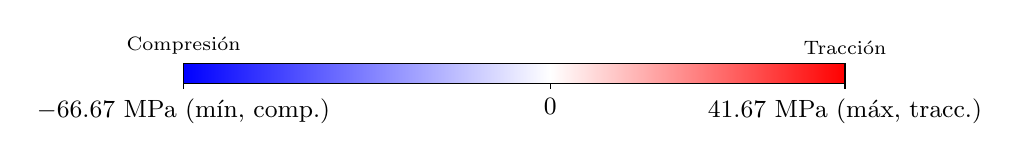
\begin{tikzpicture}[scale=0.42]
\def\barlen{20}
\def\barh{0.6}
\pgfmathsetmacro{\zeropos}{\barlen*\smin/(\smin+\smax)}
\shade[left color=blue, right color=white] (0,0) rectangle (\zeropos,\barh);
\shade[left color=white, right color=red] (\zeropos,0) rectangle (\barlen,\barh);
\draw (0,0) rectangle (\barlen,\barh);
\draw (0,0) -- (0,-0.15) node[below] {\small $-66.67$ MPa (mín, comp.)};
\draw (\zeropos,0) -- (\zeropos,-0.15) node[below] {\small $0$};
\draw (\barlen,0) -- (\barlen,-0.15) node[below] {\small $41.67$ MPa (máx, tracc.)};
\node[above] at (0,\barh) {\scriptsize Compresión};
\node[above] at (\barlen,\barh) {\scriptsize Tracción};
\end{tikzpicture}
}%
\end{center}

\vspace{1em}
\begin{center}
{%
\begin{tikzpicture}[scale=0.42]
\tikzset{joint/.style={circle, fill=black, inner sep=1.5pt}}
\tikzset{jointdef/.style={circle, fill=red!70!black, inner sep=1.3pt}}
\def\amp{100} % mismo factor que en el Modelo 1
% ===== Nodos originales =====
\coordinate (n0)  at (0,0);
\coordinate (n1)  at (4,0);
\coordinate (n2)  at (8,0);
\coordinate (n3)  at (12,0);
\coordinate (n4)  at (16,0);
\coordinate (n5)  at (20,0);
\coordinate (n6)  at (0,3);
\coordinate (n7)  at (4,3);
\coordinate (n8)  at (8,3);
\coordinate (n9)  at (12,3);
\coordinate (n10) at (16,3);
\coordinate (n11) at (20,3);

% ===== Nodos deformados (original + amp * desplazamiento) =====
\dnode{m0}{0}{0}{0.000}{0.000}
\dnode{m1}{4}{0}{-0.129}{-5.302}
\dnode{m2}{8}{0}{0.388}{-9.550}
\dnode{m3}{12}{0}{0.906}{-9.331}
\dnode{m4}{16}{0}{0.777}{-5.011}
\dnode{m5}{20}{0}{0.000}{0.000}
\dnode{m6}{0}{3}{2.439}{0.000}
\dnode{m7}{4}{3}{2.439}{-4.938}
\dnode{m8}{8}{3}{1.792}{-9.550}
\dnode{m9}{12}{3}{0.498}{-9.695}
\dnode{m10}{16}{3}{-0.797}{-5.375}
\dnode{m11}{20}{3}{-1.444}{-0.364}

% ===== Estructura original (referencia, gris punteado) =====
\draw[dashed, gray, line width=0.8pt]
  (n0)--(n1)--(n2)--(n3)--(n4)--(n5)
  (n6)--(n7)--(n8)--(n9)--(n10)--(n11)
  (n0)--(n6) (n1)--(n7) (n2)--(n8) (n3)--(n9) (n4)--(n10) (n5)--(n11)
  (n0)--(n7) (n1)--(n8) (n2)--(n9) (n3)--(n10) (n4)--(n11);

% ===== Estructura deformada (solida, coloreada) =====
\draw[thick, blue!70!black]
  (m0)--(m1)--(m2)--(m3)--(m4)--(m5)
  (m6)--(m7)--(m8)--(m9)--(m10)--(m11)
  (m0)--(m6) (m1)--(m7) (m2)--(m8) (m3)--(m9) (m4)--(m10) (m5)--(m11)
  (m0)--(m7) (m1)--(m8) (m2)--(m9) (m3)--(m10) (m4)--(m11);

% Nodos originales (fantasma) y deformados
\foreach \n in {0,...,11}{\node[joint, fill=gray!60] at (n\n) {};}
\foreach \n in {0,...,11}{\node[jointdef] at (m\n) {};}

% Apoyos (en posicion original, no se mueven)
\draw[fill=gray!40] (0,0) -- (-0.4,-0.7) -- (0.4,-0.7) -- cycle;
\draw (-0.6,-0.7) -- (0.6,-0.7);
\foreach \x in {-0.6,-0.4,-0.2,0,0.2,0.4}{\draw (\x,-0.7) -- (\x-0.15,-0.95);}
\draw[fill=gray!40] (20,0) -- (19.6,-0.7) -- (20.4,-0.7) -- cycle;
\draw (19.4,-0.7) -- (20.6,-0.7);
\foreach \x in {19.4,19.6,19.8,20.0,20.2,20.4}{\draw (\x,-0.7) -- (\x-0.15,-0.95);}

% Etiqueta del desplazamiento maximo (nodo 8)
\draw[-{Latex[length=2mm]}, thin] (m8) -- ++(1.2,3.3)
  node[right] {\small $|\vec{u}|_{8} \approx 9.72\,\text{mm}$};
\end{tikzpicture}

\vspace{0.3em}
{\small
\tikz[baseline=-0.5ex]\draw[dashed, gray, line width=1pt] (0,0)--(0.5,0); \; Estructura original \qquad
\tikz[baseline=-0.5ex]\draw[thick, blue!70!black] (0,0)--(0.5,0); \; Deformada (amplificada $\times\,100$)
}
}%
\end{center}

\end{desarrollo}

\begin{desarrollo}{Puente 3D}
    Bueno para este caso el mas simple era el 2 cantidad de nodos pero el que era mas interesante era el 1 por ende hare el 1, es basicamente una copia pero hay que conectar las copias entre ellas, las conectare en cruz para asi poder 

    % ================= VISTA LATERAL (XY) =================
\begin{center}
\begin{tikzpicture}[scale=0.42]
\tikzset{joint/.style={circle, fill=black, inner sep=1pt}}
% Nodos (solo los de los planos frontal/posterior)
\coordinate (n0) at (0,0);
\coordinate (n1) at (2,0);
\coordinate (n2) at (2,1);
\coordinate (n3) at (4,0);
\coordinate (n4) at (4,2);
\coordinate (n5) at (6,0);
\coordinate (n6) at (6,2.75);
\coordinate (n7) at (8,0);
\coordinate (n8) at (8,3.25);
\coordinate (n9) at (10,0);
\coordinate (n10) at (10,3.5);
\coordinate (n11) at (12,0);
\coordinate (n12) at (12,3.25);
\coordinate (n13) at (14,0);
\coordinate (n14) at (14,2.75);
\coordinate (n15) at (16,0);
\coordinate (n16) at (16,2);
\coordinate (n17) at (18,0);
\coordinate (n18) at (18,1);
\coordinate (n19) at (20,0);
\coordinate (n20) at (0,0);
\coordinate (n21) at (2,0);
\coordinate (n22) at (2,1);
\coordinate (n23) at (4,0);
\coordinate (n24) at (4,2);
\coordinate (n25) at (6,0);
\coordinate (n26) at (6,2.75);
\coordinate (n27) at (8,0);
\coordinate (n28) at (8,3.25);
\coordinate (n29) at (10,0);
\coordinate (n30) at (10,3.5);
\coordinate (n31) at (12,0);
\coordinate (n32) at (12,3.25);
\coordinate (n33) at (14,0);
\coordinate (n34) at (14,2.75);
\coordinate (n35) at (16,0);
\coordinate (n36) at (16,2);
\coordinate (n37) at (18,0);
\coordinate (n38) at (18,1);
\coordinate (n39) at (20,0);
% Plano frontal z=0
\draw[thick, blue!65!black]
  (n0)--(n1) (n0)--(n2) (n1)--(n2) (n1)--(n3) (n2)--(n3) (n2)--(n4) (n3)--(n4) (n3)--(n5) (n3)--(n6) (n4)--(n6) (n5)--(n6) (n5)--(n7) (n6)--(n7) (n6)--(n8) (n7)--(n8) (n7)--(n9) (n7)--(n10) (n8)--(n10) (n9)--(n10) (n9)--(n11) (n10)--(n11) (n10)--(n12) (n11)--(n12) (n11)--(n13) (n11)--(n14) (n12)--(n14) (n13)--(n14) (n13)--(n15) (n14)--(n15) (n14)--(n16) (n15)--(n16) (n15)--(n17) (n15)--(n18) (n16)--(n18) (n17)--(n18) (n17)--(n19) (n18)--(n19);
% Plano posterior z=3 (id�ntico en XY, se dibuja superpuesto)
\draw[thick, dashed, red!70!black]
  (n20)--(n21) (n20)--(n22) (n21)--(n22) (n21)--(n23) (n22)--(n23) (n22)--(n24) (n23)--(n24) (n23)--(n25) (n23)--(n26) (n24)--(n26) (n25)--(n26) (n25)--(n27) (n26)--(n27) (n26)--(n28) (n27)--(n28) (n27)--(n29) (n27)--(n30) (n28)--(n30) (n29)--(n30) (n29)--(n31) (n30)--(n31) (n30)--(n32) (n31)--(n32) (n31)--(n33) (n31)--(n34) (n32)--(n34) (n33)--(n34) (n33)--(n35) (n34)--(n35) (n34)--(n36) (n35)--(n36) (n35)--(n37) (n35)--(n38) (n36)--(n38) (n37)--(n38) (n37)--(n39) (n38)--(n39);
% Apoyos (coinciden para ambos planos en esta vista)
\begin{scope}[shift={(n0)}]
\draw[fill=gray!40] (0,0) -- (-0.4,-0.7) -- (0.4,-0.7) -- cycle;
\draw (-0.6,-0.7) -- (0.6,-0.7);
\foreach \xx in {-0.6,-0.4,-0.2,0,0.2,0.4}{\draw (\xx,-0.7) -- (\xx-0.15,-0.95);}
\end{scope}
\begin{scope}[shift={(n19)}]
\draw[fill=gray!40] (0,0) -- (-0.4,-0.7) -- (0.4,-0.7) -- cycle;
\draw (-0.6,-0.7) -- (0.6,-0.7);
\foreach \xx in {-0.6,-0.4,-0.2,0,0.2,0.4}{\draw (\xx,-0.7) -- (\xx-0.15,-0.95);}
\end{scope}
% Carga (25 kN en cada plano, coinciden en esta vista)
\draw[-{Latex[length=3mm]}, thick, black] (n9) -- ++(0,-1.5) node[below] {\small $2\times 25\,\text{kN}$};
\end{tikzpicture}
\end{center}

% ================= VISTA SUPERIOR (XZ) =================
\begin{center}
\begin{tikzpicture}[scale=0.42]
\tikzset{joint/.style={circle, fill=black, inner sep=1pt}}
% Nodos usados por el arriostramiento (vista XZ)
\coordinate (p0) at (0,0);
\coordinate (p1) at (2,0);
\coordinate (p2) at (2,0);
\coordinate (p3) at (4,0);
\coordinate (p4) at (4,0);
\coordinate (p5) at (6,0);
\coordinate (p6) at (6,0);
\coordinate (p7) at (8,0);
\coordinate (p8) at (8,0);
\coordinate (p9) at (10,0);
\coordinate (p10) at (10,0);
\coordinate (p11) at (12,0);
\coordinate (p12) at (12,0);
\coordinate (p13) at (14,0);
\coordinate (p14) at (14,0);
\coordinate (p15) at (16,0);
\coordinate (p16) at (16,0);
\coordinate (p17) at (18,0);
\coordinate (p18) at (18,0);
\coordinate (p19) at (20,0);
\coordinate (p20) at (0,3);
\coordinate (p21) at (2,3);
\coordinate (p22) at (2,3);
\coordinate (p23) at (4,3);
\coordinate (p24) at (4,3);
\coordinate (p25) at (6,3);
\coordinate (p26) at (6,3);
\coordinate (p27) at (8,3);
\coordinate (p28) at (8,3);
\coordinate (p29) at (10,3);
\coordinate (p30) at (10,3);
\coordinate (p31) at (12,3);
\coordinate (p32) at (12,3);
\coordinate (p33) at (14,3);
\coordinate (p34) at (14,3);
\coordinate (p35) at (16,3);
\coordinate (p36) at (16,3);
\coordinate (p37) at (18,3);
\coordinate (p38) at (18,3);
\coordinate (p39) at (20,3);
\coordinate (p40) at (10,1.5);
% Lineas de referencia de cada plano (z=0 y z=3)
\draw[thin, gray] (0,0) -- (20,0);
\draw[thin, gray] (0,3) -- (20,3);
% Arriostramiento (postes, cruzadas, anti-mecanismo, nodo 40)
\draw[thick, teal!70!black]
  (p0)--(p20) (p1)--(p21) (p3)--(p23) (p4)--(p24) (p5)--(p25) (p6)--(p26) (p7)--(p27) (p8)--(p28) (p9)--(p29) (p10)--(p40) (p40)--(p30) (p11)--(p31) (p12)--(p32) (p13)--(p33) (p14)--(p34) (p15)--(p35) (p16)--(p36) (p17)--(p37) (p19)--(p39) (p0)--(p21) (p1)--(p20) (p1)--(p23) (p3)--(p21) (p3)--(p25) (p5)--(p23) (p5)--(p27) (p7)--(p25) (p7)--(p29) (p9)--(p27) (p9)--(p31) (p11)--(p29) (p11)--(p33) (p13)--(p31) (p13)--(p35) (p15)--(p33) (p15)--(p37) (p17)--(p35) (p17)--(p39) (p19)--(p37) (p6)--(p22) (p2)--(p26) (p4)--(p26) (p6)--(p24) (p6)--(p28) (p8)--(p26) (p8)--(p30) (p10)--(p28) (p10)--(p32) (p12)--(p30) (p12)--(p34) (p14)--(p32) (p14)--(p36) (p16)--(p34) (p14)--(p38) (p18)--(p34) (p32)--(p8) (p28)--(p12) (p30)--(p6) (p30)--(p14) (p10)--(p34) (p10)--(p26) (p40)--(p9) (p40)--(p29) (p40)--(p8) (p40)--(p12);
% Nodos
\foreach \p in {0,1,2,3,4,5,6,7,8,9,10,11,12,13,14,15,16,17,18,19,20,21,22,23,24,25,26,27,28,29,30,31,32,33,34,35,36,37,38,39,40}{\node[joint] at (p\p) {};}
% Apoyos (triangulos en las 4 esquinas)
\node[regular polygon, regular polygon sides=3, fill=gray!50, minimum size=5pt, inner sep=0pt] at (p0) {};
\node[regular polygon, regular polygon sides=3, fill=gray!50, minimum size=5pt, inner sep=0pt] at (p19) {};
\node[regular polygon, regular polygon sides=3, fill=gray!50, minimum size=5pt, inner sep=0pt] at (p20) {};
\node[regular polygon, regular polygon sides=3, fill=gray!50, minimum size=5pt, inner sep=0pt] at (p39) {};
% Cargas
\node[circle, fill=red!70!black, inner sep=1.3pt] at (p9) {};
\node[right=2pt] at (p9) {\tiny 25 kN $\downarrow$};
\node[circle, fill=red!70!black, inner sep=1.3pt] at (p29) {};
\node[right=2pt] at (p29) {\tiny 25 kN $\downarrow$};
\node[below] at (10,-0.3) {\small $x$ [m]};
\node[left] at (-0.3,1.5) {\small $z$ [m]};
\end{tikzpicture}
\end{center}

% ================= VISTA ISOMETRICA =================
\begin{center}
\begin{tikzpicture}[scale=0.32]
\tikzset{joint/.style={circle, fill=black, inner sep=0.8pt}}
% Nodos proyectados (proyeccion cabinet, angulo 45, k=0.5)
\coordinate (q0) at (0,0);
\coordinate (q1) at (2,0);
\coordinate (q2) at (2,1);
\coordinate (q3) at (4,0);
\coordinate (q4) at (4,2);
\coordinate (q5) at (6,0);
\coordinate (q6) at (6,2.75);
\coordinate (q7) at (8,0);
\coordinate (q8) at (8,3.25);
\coordinate (q9) at (10,0);
\coordinate (q10) at (10,3.5);
\coordinate (q11) at (12,0);
\coordinate (q12) at (12,3.25);
\coordinate (q13) at (14,0);
\coordinate (q14) at (14,2.75);
\coordinate (q15) at (16,0);
\coordinate (q16) at (16,2);
\coordinate (q17) at (18,0);
\coordinate (q18) at (18,1);
\coordinate (q19) at (20,0);
\coordinate (q20) at (1.061,1.061);
\coordinate (q21) at (3.061,1.061);
\coordinate (q22) at (3.061,2.061);
\coordinate (q23) at (5.061,1.061);
\coordinate (q24) at (5.061,3.061);
\coordinate (q25) at (7.061,1.061);
\coordinate (q26) at (7.061,3.811);
\coordinate (q27) at (9.061,1.061);
\coordinate (q28) at (9.061,4.311);
\coordinate (q29) at (11.06,1.061);
\coordinate (q30) at (11.06,4.561);
\coordinate (q31) at (13.06,1.061);
\coordinate (q32) at (13.06,4.311);
\coordinate (q33) at (15.06,1.061);
\coordinate (q34) at (15.06,3.811);
\coordinate (q35) at (17.06,1.061);
\coordinate (q36) at (17.06,3.061);
\coordinate (q37) at (19.06,1.061);
\coordinate (q38) at (19.06,2.061);
\coordinate (q39) at (21.06,1.061);
\coordinate (q40) at (10.53,4.03);
% Arriostramiento (se dibuja primero, mas discreto)
\draw[thin, teal!60!black]
  (q0)--(q20) (q1)--(q21) (q3)--(q23) (q4)--(q24) (q5)--(q25) (q6)--(q26) (q7)--(q27) (q8)--(q28) (q9)--(q29) (q10)--(q40) (q40)--(q30) (q11)--(q31) (q12)--(q32) (q13)--(q33) (q14)--(q34) (q15)--(q35) (q16)--(q36) (q17)--(q37) (q19)--(q39) (q0)--(q21) (q1)--(q20) (q1)--(q23) (q3)--(q21) (q3)--(q25) (q5)--(q23) (q5)--(q27) (q7)--(q25) (q7)--(q29) (q9)--(q27) (q9)--(q31) (q11)--(q29) (q11)--(q33) (q13)--(q31) (q13)--(q35) (q15)--(q33) (q15)--(q37) (q17)--(q35) (q17)--(q39) (q19)--(q37) (q6)--(q22) (q2)--(q26) (q4)--(q26) (q6)--(q24) (q6)--(q28) (q8)--(q26) (q8)--(q30) (q10)--(q28) (q10)--(q32) (q12)--(q30) (q12)--(q34) (q14)--(q32) (q14)--(q36) (q16)--(q34) (q14)--(q38) (q18)--(q34) (q32)--(q8) (q28)--(q12) (q30)--(q6) (q30)--(q14) (q10)--(q34) (q10)--(q26) (q40)--(q9) (q40)--(q29) (q40)--(q8) (q40)--(q12);
% Plano posterior z=3
\draw[thick, red!70!black]
  (q20)--(q21) (q20)--(q22) (q21)--(q22) (q21)--(q23) (q22)--(q23) (q22)--(q24) (q23)--(q24) (q23)--(q25) (q23)--(q26) (q24)--(q26) (q25)--(q26) (q25)--(q27) (q26)--(q27) (q26)--(q28) (q27)--(q28) (q27)--(q29) (q27)--(q30) (q28)--(q30) (q29)--(q30) (q29)--(q31) (q30)--(q31) (q30)--(q32) (q31)--(q32) (q31)--(q33) (q31)--(q34) (q32)--(q34) (q33)--(q34) (q33)--(q35) (q34)--(q35) (q34)--(q36) (q35)--(q36) (q35)--(q37) (q35)--(q38) (q36)--(q38) (q37)--(q38) (q37)--(q39) (q38)--(q39);
% Plano frontal z=0 (al frente, se dibuja al final)
\draw[thick, blue!65!black]
  (q0)--(q1) (q0)--(q2) (q1)--(q2) (q1)--(q3) (q2)--(q3) (q2)--(q4) (q3)--(q4) (q3)--(q5) (q3)--(q6) (q4)--(q6) (q5)--(q6) (q5)--(q7) (q6)--(q7) (q6)--(q8) (q7)--(q8) (q7)--(q9) (q7)--(q10) (q8)--(q10) (q9)--(q10) (q9)--(q11) (q10)--(q11) (q10)--(q12) (q11)--(q12) (q11)--(q13) (q11)--(q14) (q12)--(q14) (q13)--(q14) (q13)--(q15) (q14)--(q15) (q14)--(q16) (q15)--(q16) (q15)--(q17) (q15)--(q18) (q16)--(q18) (q17)--(q18) (q17)--(q19) (q18)--(q19);
% Nodos
\foreach \n in {0,...,40}{\node[joint] at (q\n) {};}
% Apoyos
\begin{scope}[shift={(0,0)}]
\draw[fill=gray!40] (0,0) -- (-0.3,-0.55) -- (0.3,-0.55) -- cycle;
\end{scope}
\begin{scope}[shift={(20,0)}]
\draw[fill=gray!40] (0,0) -- (-0.3,-0.55) -- (0.3,-0.55) -- cycle;
\end{scope}
\begin{scope}[shift={(1.061,1.061)}]
\draw[fill=gray!40] (0,0) -- (-0.3,-0.55) -- (0.3,-0.55) -- cycle;
\end{scope}
\begin{scope}[shift={(21.06,1.061)}]
\draw[fill=gray!40] (0,0) -- (-0.3,-0.55) -- (0.3,-0.55) -- cycle;
\end{scope}
% Cargas
\draw[-{Latex[length=2.5mm]}, thick, black] (10,0) -- ++(0,-1.1) node[below] {\tiny $25\,\text{kN}$};
\draw[-{Latex[length=2.5mm]}, thick, black] (11.06,1.061) -- ++(0,-1.1) node[below] {\tiny $25\,\text{kN}$};
\end{tikzpicture}
\end{center}
\end{desarrollo}
\lstinputlisting[style=pythonstyle, caption={FEM para elementos unidimensionales}, label={lst:solver}]{T1/T1_1.py}



